\subsection{Support Vector Machines}
\label{svm}
\underline{Grundidee}: Finde die Hyperebene $h_0$, die die Klassen trennt und den größtmöglichen Abstand zu den nächsten Trainingsdatenpunkten hat. Die jeweils nächsten Datenpunkte werden als \emph{Support Vectors} bezeichnet.\\

Anders als bei der logistischen Regression wird bei SVMs die Klassifikationsgrenze \emph{explizit} gelernt und nicht \emph{implizit} berechnet.\\
\begin{figure*}[!h]    
    \centering
    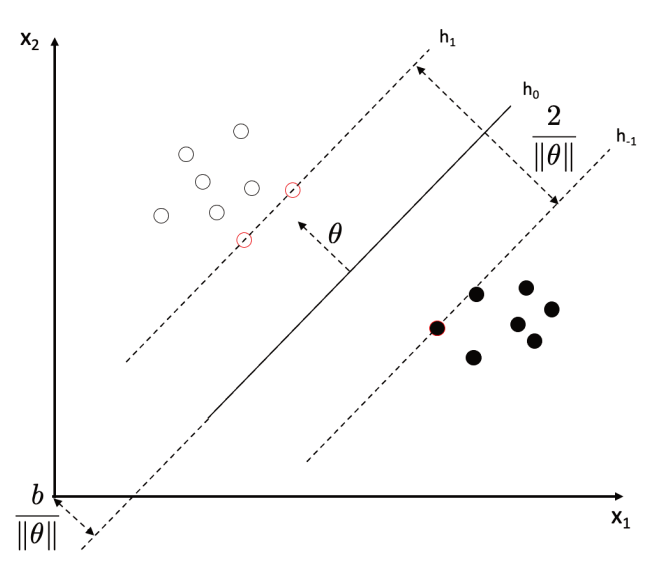
\includegraphics[width=0.5\textwidth]{supervisedLearning/svm.png}
    \caption{Support Vector Machines}
    \label{fig:svm}
\end{figure*}

\begin{itemize}
    \item $\Theta$ ist der Normalenvektor der Hyperebene
    \item $b$ ist der Abstand der Hyperebene zum Ursprung\\
\end{itemize}

Optimierungsproblem der \textbf{Hard-Margin SVM} (Klassen sind linear eindeutig linear trennbar):
\begin{equation*}
    \begin{split}
        \min \| \Theta \|\\
        \text{s.t. } y(\Theta^Tx-bs)\geq 1 \text{ für } (x,y) \in D
    \end{split}
\end{equation*}

Alternativ: Maximiere den Abstand zwischen den Hyperebenen $h_1$ und $h_{-1}\rightarrow \text{max}\frac{2}{\|\Theta\|}$\\

Für die Hyperebene $h_0$ sowie die parallel verlaufenden Ebenen $h_1$ und $h_{-1}$ gelten:
\begin{equation*}
    \begin{split}
        h_0: \Theta^Tx-b=0\\
        h_1: \Theta^Tx-b=1\\
        h_{-1}: \Theta^Tx-b=-1
    \end{split}
\end{equation*}

Lineare Separierbarkeit ist in der Praxis selten gegeben. \emph{Hard-Margin SVM} besitzt dann keine zulässige Lösung (undefiniert). Daher wird die \textbf{Soft-Margin SVM} verwendet, die Ausreißer zulässt:

\begin{equation*}
    \min C\| \Theta \|^2 + \frac{1}{m}\underbrace{\sum_{i=1}^{m}\max(0,1-y^{(i)}(\Theta^Tx^{(i)}-b))}_{\text{Hinge-Kostenfunktion} (L^\text{Hinge})}    
\end{equation*}

\begin{itemize}
    \item $C\in\mathbb{R}^{>0}$ ist ein Regularisierungsparameter ($C\|\Theta\|^2$ ist identisch zum \emph{Tikhonov-Regularisierer}):
    \begin{itemize}
        \item kleines $C$ $\rightarrow$ ähnliche (gleiche?) Ergebnisse wie \emph{Hard-Margin SVM}
        \item großes $C$ $\rightarrow$ Klassifikator wird toleranter ggü. Abweichungen von linearer Separierbarkeit von $D$ 
    \end{itemize}
    \item $L^\text{Hinge}$ ist die Kostenfunktion, die die Verletzung der Margin-Kontraints bestraft: Bei korrekter Klassifikation wird $L^\text{Hinge}=0$
    \item $y^{(i)}(\Theta^Tx^{(i)}-b)$ ist der Abstand des $i$-ten Datenpunkts zur Hyperebene
\end{itemize}

Anwendung auf nicht-lineare Daten durch \textbf{Kernel-Trick}: Anstatt (rechenaufwändig) Merkmale zu erweitern (s. lineare/logistische Regression) kann die Transformation implizit durch einen Kernel $k(x^{(i)},x^{(j)})$ erfolgen. Gebräuchliche Kernel sind:\\

\begin{itemize}
    \item $k^d_{\text{poly-h}}(x, x')=(x^Tx')^d \rightarrow$ homogener polynomieller Kernel zu Grad $d > 0$
    \item $k^{d,r}_{\text{poly-i}}(x, x')=(x^Tx'+r)^d \rightarrow$ inhomogener polynomieller Kernel zu Grad $d > 0$ mit $r\in\mathbb{R}$
    \item $k^{\gamma}_{\text{rbf}}(x, x')=e^{-\gamma\|x-x'\|^2} \rightarrow$ \emph{Gaußscher Kernel}, Radiale Basisfunktion mit $\gamma > 0$
\end{itemize}

\begin{figure*}[!h]    
    \centering
    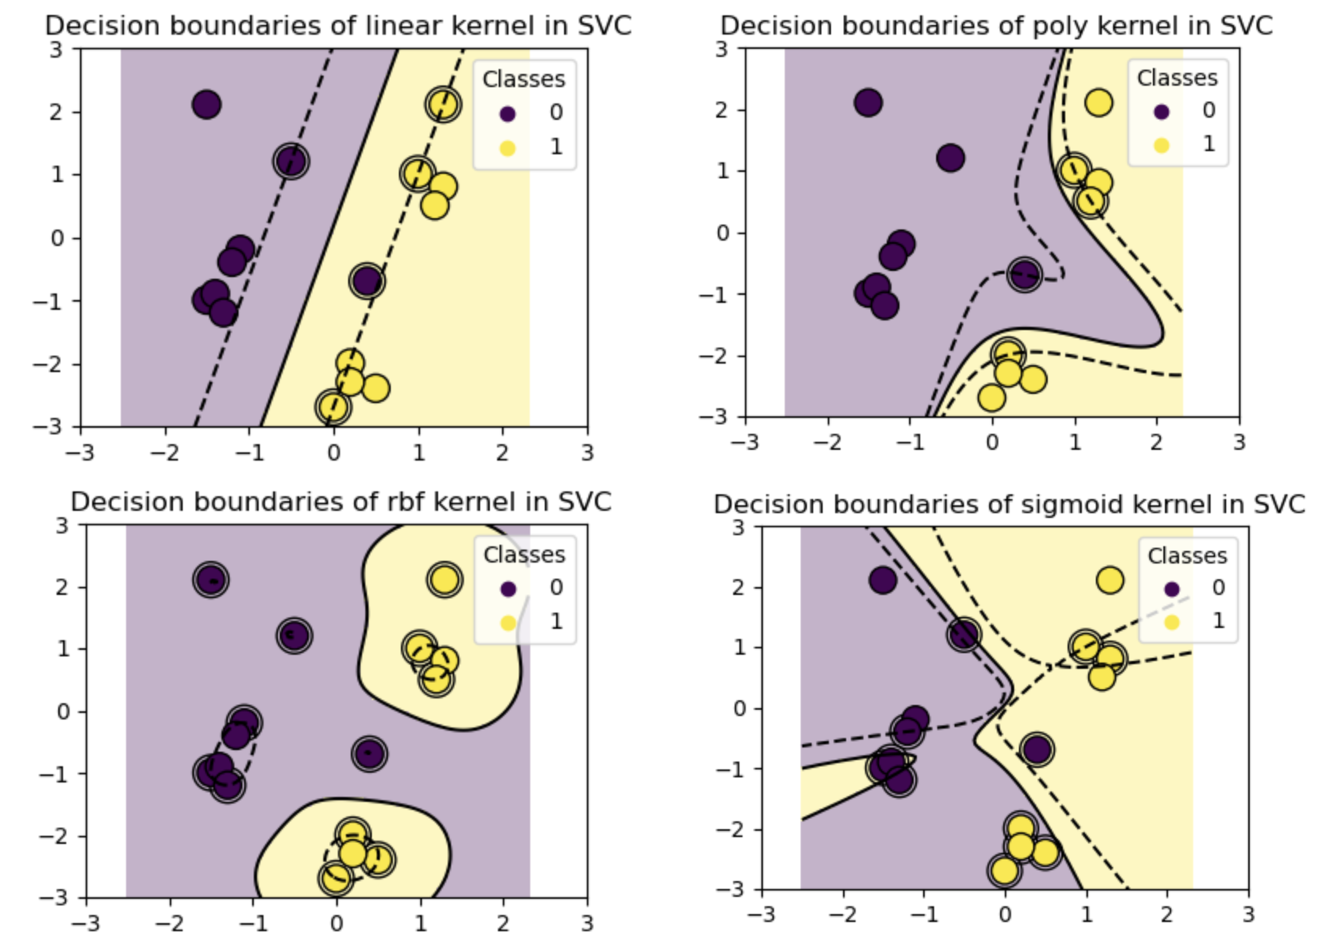
\includegraphics[width=0.5\textwidth]{supervisedLearning/kernel-svm-example.png}
    \caption{Kernel-Unterschiede}
    \label{fig:kernelOverview}
\end{figure*}